\documentclass[11pt]{article}

\usepackage[margin=0.68in]{geometry}
\usepackage{amssymb}
\usepackage{booktabs}
\usepackage[american]{circuitikz}
\usepackage{enumitem}
\usepackage{fancyhdr}
\usepackage{graphicx}
\usepackage[table]{xcolor}
\usepackage[hidelinks]{hyperref}
\usepackage{listings}
\usepackage{microtype}
\usepackage{tabularx}
\usepackage{tikz}
\usepackage{titlesec}
\usetikzlibrary{positioning}
\graphicspath{{docs/lessons/assets/}{../assets/}}

\definecolor{AdkBlue}{gray}{0.125}
\definecolor{AdkRed}{gray}{0}
\definecolor{AdkGreen}{gray}{0.315}
\definecolor{CodeGray}{gray}{0.969}
\hypersetup
{
    pdftitle={ADK Lesson 006: Deterministic Simon},
    pdfauthor={Kevin Shanahan},
    pdfsubject={Four-button Simon project with deterministic state, replay, PRNG, light, and sound},
    pdflang={en-US}
}
\pagestyle{fancy}
\fancyhf{}
\lhead{\textsc{ADK Lesson 006}}
\rhead{Deterministic Simon}
\cfoot{\thepage}
\setlength{\headheight}{14pt}
\setlength{\parindent}{0pt}
\setlength{\parskip}{5pt}
\setlist{nosep,leftmargin=1.45em}
\titleformat{\section}{\Large\bfseries\color{AdkBlue}}{\thesection}{0.5em}{}
\titleformat{\subsection}{\large\bfseries\color{AdkBlue}}{\thesubsection}{0.5em}{}
\lstdefinestyle{adkcpp}
{
    language=C++,
    backgroundcolor=\color{CodeGray},
    basicstyle=\ttfamily\small,
    keywordstyle=\color{AdkBlue}\bfseries,
    commentstyle=\color{AdkGreen},
    columns=fullflexible,
    keepspaces=true,
    showstringspaces=false,
    frame=single,
    rulecolor=\color{black!20},
    breaklines=true,
    tabsize=4
}
\newcommand{\checkbox}{\(\square\)}
\newcommand{\blank}[1]{\rule{#1}{0.4pt}}
\newcommand{\warningbox}[1]{%
  \begin{center}
  \fcolorbox{AdkRed}{AdkRed!6}{\parbox{0.91\linewidth}{\textbf{\color{AdkRed}Safety checkpoint.} #1}}
  \end{center}}
\newcommand{\evidencebox}[1]{%
  \begin{center}
  \fcolorbox{AdkBlue}{AdkBlue!5}{\parbox{0.91\linewidth}{#1}}
  \end{center}}

\begin{document}

\begin{center}
  {\Huge\bfseries Deterministic Simon}\\[4pt]
  {\Large Four buttons, four cues, RGB status, and sound --- Mega 2560}\\[8pt]
  \textit{If seed, configuration, time, and input match, every observable must match.}
\end{center}

\begin{tabularx}{\linewidth}{@{}>{\bfseries}l X >{\bfseries}l X@{}}
Lesson & 006 --- integration project & Time & 150--210 minutes\\
Engine & host verified & Hardware adapter & experimental\\
Evidence & replay, fault tests, measurements & Board & Arduino Mega 2560\\
Safety & E1: USB-powered indicators, controls, and passive piezo only\\
\end{tabularx}

\section{Mission}

Build a memory game that plays a sequence of four neutral cues, accepts one
debounced button at a time, grows the sequence, and reports success or failure
with light and sound. First prove the state machine with a fixed cue source.
Then prove the versioned PRNG. Only then connect hardware.

By the end, you can:

\begin{itemize}
  \item compose four \texttt{Button}s, four \texttt{MonoLed}s, one
        \texttt{RgbLed}, and a \texttt{PiezoSounder} around \texttt{Simon};
  \item pack complete input into masks without depending on button update order;
  \item trace every \texttt{SimonPhase}, deadline, and terminal outcome;
  \item reproduce a game from algorithm version, seed, configuration, timestamps,
        and input observations;
  \item reject simultaneous input and injected source failure deterministically;
  \item calculate LED current and record a Mega 2560 hardware acceptance result.
\end{itemize}

\warningbox{Disconnect USB and every other power source before changing wiring.
Every LED die needs its own 330\(\Omega\) series resistor: seven resistors total
for four cue LEDs plus three RGB channels. Use a passive piezo element, not a
speaker or an unidentified active module; place 100\(\Omega\) in series. Never
connect an output to 5\,V or GND directly. Stop for heat, odor, board resets,
distortion, or unexpected brightness.}

\evidencebox{\textbf{Neutral-cue boundary.} This project is a memory game.
\texttt{CueId} values have no launcher, ignition, continuity, or radio meaning.
Do not connect the project to a firing system, initiator, transmitter, captured
remote, relay, or other energetic load. Later show-cue work remains an inert
host/indicator simulation and provides no RF replay or launcher interface.}

\section{Composition, not inheritance}

\begin{center}
% ADK visual: pencil
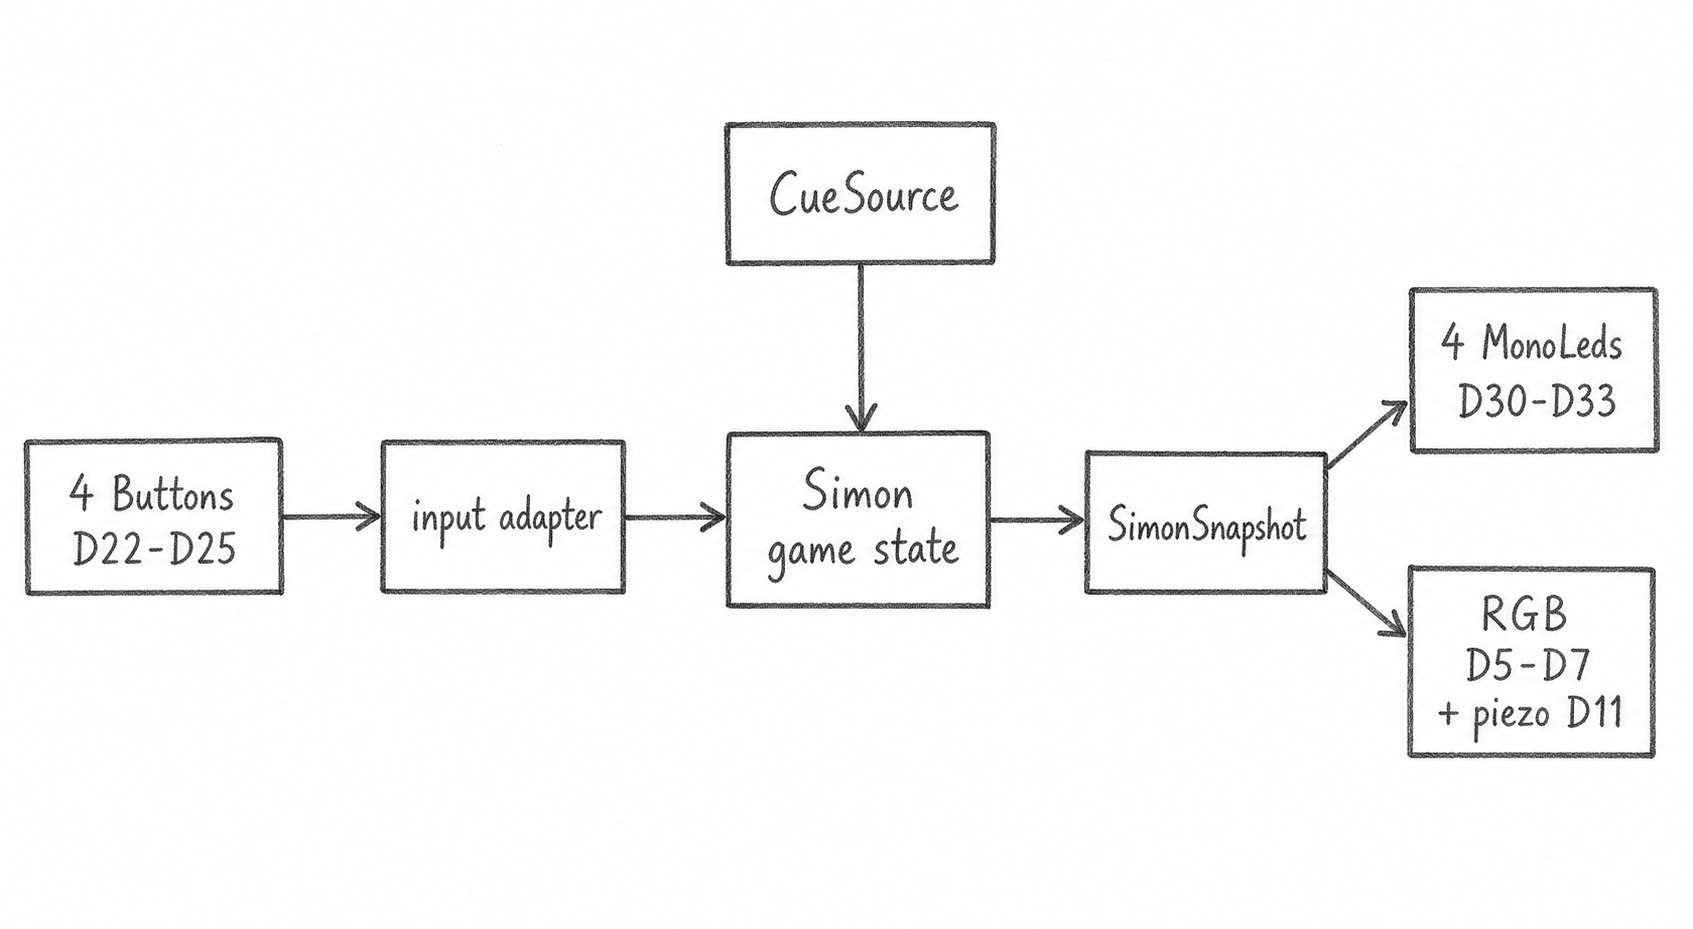
\includegraphics[width=\linewidth,height=0.28\textheight,keepaspectratio]
  {006-simon-composition-pencil.png}
\end{center}

\texttt{Simon} owns no GPIO and reads no clock. The adapter samples all buttons,
then presents one immutable \texttt{SimonInput}. Output adapters consume one
snapshot after the update. \texttt{RgbLed} composes three supported
\texttt{PwmOutput}s and records the three channel/resistor specifications.
\texttt{PiezoSounder} owns its pin and timer claim. The canonical
\texttt{examples/Lesson006Simon} sketch uses this complete composition. A
separate \texttt{MonoLed} on D13 pulses for 250\,ms after every resource is
acquired, followed by 750\,ms with D13 and all game outputs dark. Button
sampling and game behavior begin only after that separator.

\section{Orientation drawing}

\begin{figure}[ht]
  \centering
  % ADK visual: pencil
  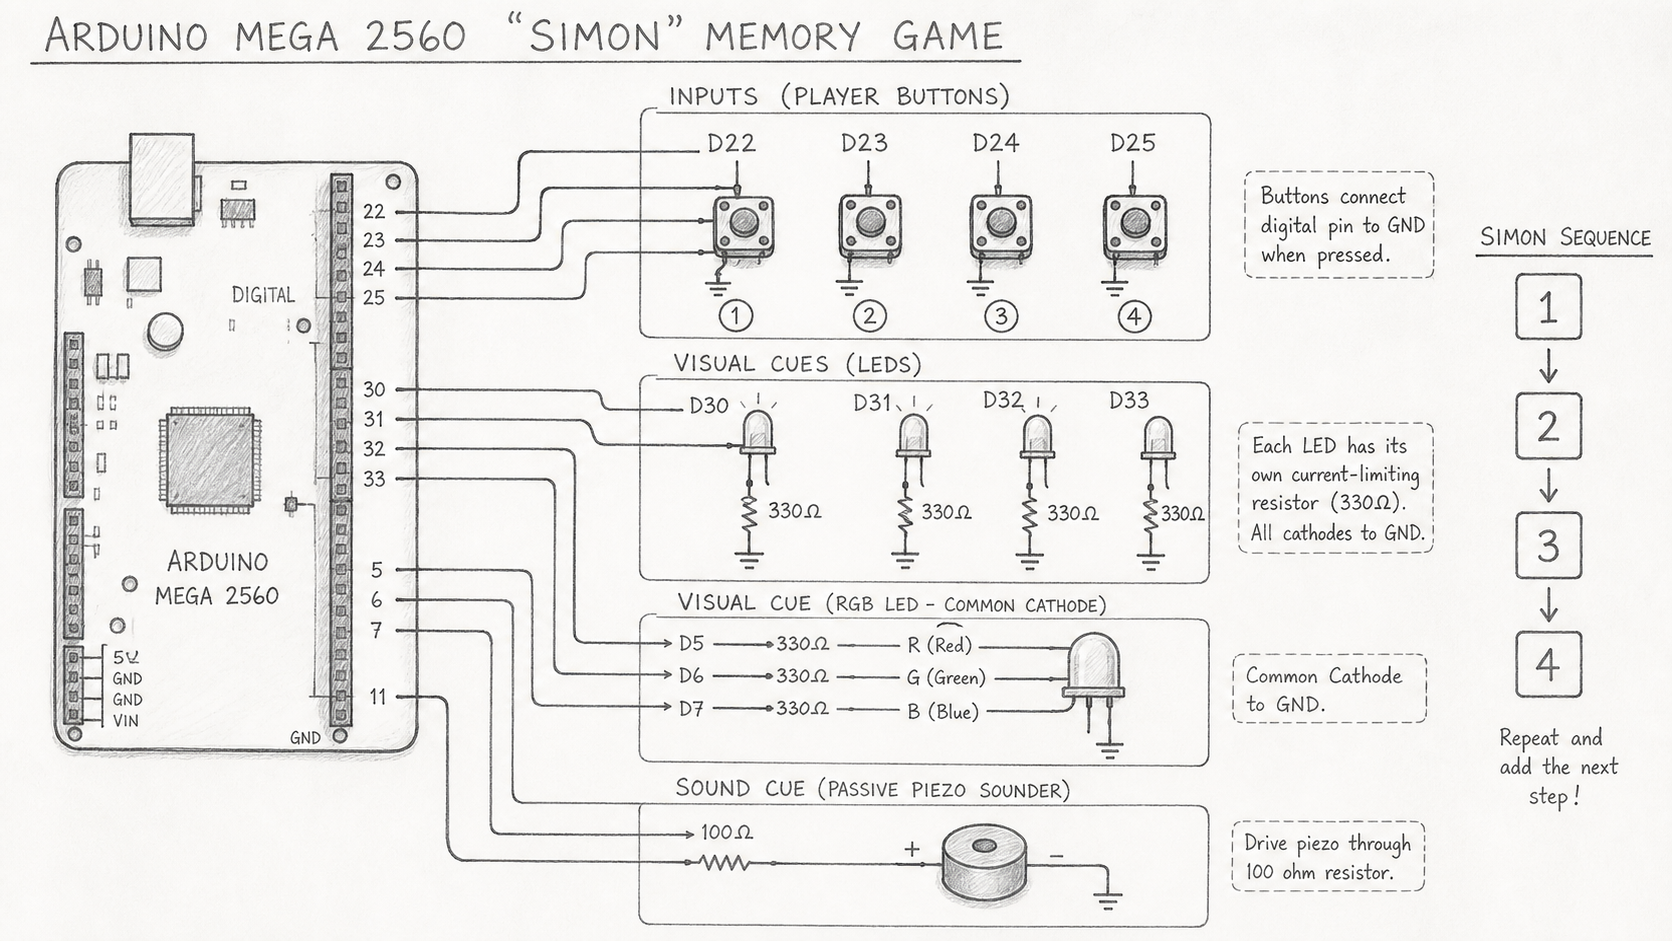
\includegraphics[width=\linewidth]{006-simon-pencil.png}
  \caption{Conceptual pencil orientation for the complete control panel. This
  drawing helps locate functional groups, but it is \textbf{not authoritative
  wiring guidance}: board-header geometry, breadboard connectivity, component
  lead order, and polarity may be simplified. Build and verify only from the
  exact schematics, pin table, part datasheets, and unpowered continuity checks
  below.}
\end{figure}

\section{Exact electrical circuit}

\textbf{Pin assignment.}

\begin{center}
\small
\begin{tabularx}{\linewidth}{@{}l l X l@{}}
\toprule
Function & Mega pins & Connection & Policy\\
\midrule
acquisition & D13 & built-in LED & 250\,ms pulse after successful initialization\\
buttons 1--4 & D22--D25 & pin \(\rightarrow\) switch \(\rightarrow\) GND & internal pull-up\\
cue LEDs 1--4 & D30--D33 & pin \(\rightarrow330\,\Omega\rightarrow\) anode; cathode \(\rightarrow\) GND & active-high\\
RGB R/G/B & D5/D6/D7 & pin \(\rightarrow330\,\Omega\rightarrow\) anode; common cathode \(\rightarrow\) GND & PWM\\
passive piezo & D11 & pin \(\rightarrow100\,\Omega\rightarrow\) piezo \(+\); piezo \(-\rightarrow\) GND & tone\\
\bottomrule
\end{tabularx}
\end{center}

\begin{center}
% ADK visual: schematic
\begin{circuitikz}[american voltages,scale=.82,transform shape]
  \foreach \y/\pin/\n in {6.0/22/1,4.8/23/2,3.6/24/3,2.4/25/4}
  {
    \draw (0,\y) node[left]{D\pin\ \texttt{INPUT\_PULLUP}}
      to[short,o-] (2.4,\y) to[nos,l={button \n}] (4.8,\y)
      -- (5.5,\y);
  }
  \draw (5.5,2.4) -- (5.5,6.0) -- (5.5,1.8) node[ground]{};

  \foreach \y/\pin/\n in {6.0/30/1,4.8/31/2,3.6/32/3,2.4/33/4}
  {
    \draw (7.0,\y) node[left]{D\pin}
      to[short,o-] (7.6,\y) to[R,l={$330\,\Omega$}] (9.5,\y)
      to[leD,l={cue \n}] (11.4,\y) -- (12.1,\y);
  }
  \draw (12.1,2.4) -- (12.1,6.0) -- (12.1,1.8) node[ground]{};
\end{circuitikz}
\end{center}

\begin{center}
% ADK visual: schematic
\begin{circuitikz}[american voltages,scale=.82,transform shape]
  \foreach \y/\pin/\c in {4.0/5/R,2.8/6/G,1.6/7/B}
  {
    \draw (0,\y) node[left]{D\pin\ PWM}
      to[short,o-] (.7,\y) to[R,l={$330\,\Omega$}] (2.6,\y)
      to[leD,l={RGB \c}] (4.8,\y) -- (5.5,\y);
  }
  \draw (5.5,1.6) -- (5.5,4.0) -- (5.5,1.0)
        node[below,align=center]{common cathode} node[ground]{};
  \draw (7.1,2.8) node[left]{D11} to[short,o-] (7.8,2.8)
        to[R,l={$100\,\Omega$}] (9.6,2.8)
        to[piezoelectric,l={passive piezo}] (11.7,2.8)
        -- (12.3,2.8) -- (12.3,2.2) node[ground]{};
\end{circuitikz}
\end{center}

\textbf{The schematics are literal.} Verify RGB package pinout from its
datasheet; lead order is not universal. A common-anode RGB part requires
different wiring and inverted duty semantics. Four-pin tactile switches often
join same-side legs internally; find the contacts that change with a continuity
meter while unpowered. All ground symbols join Mega GND.

\textbf{Finite shutdown.} Successful resource acquisition simultaneously
begins the D13 pulse and an input-independent 120-second deadline. Game behavior
therefore begins 1 second into that interval. At expiry the sketch stops the
tone and commands every light inactive, preserves that observable inactive
state for 250 ms, then shuts down endpoints in reverse acquisition order.
D5--D7, D11, D13, D22--D25, and D30--D33 are then inputs/high impedance; the
loop remains halted until upload or reset. Buttons never control this deadline,
so a near-simultaneous press remains chord evidence only.

\subsection{Current budget}

For each LED channel,
\[
    I=\frac{V_{OH}-V_f}{330\,\Omega}.
\]
With a measured loaded \(V_{OH}=4.8\) V and red \(V_f=2.0\) V, the example is
8.5 mA. Measure or obtain \(V_f\) for each actual die. The normal cue design
lights one cue LED; the RGB status can light three channels. Calculate the
worst commanded simultaneous current, then compare it with every applicable
per-pin, port-group, and package limit in the ATmega2560 datasheet:

\[
 I_{\rm worst}=I_{\rm D13}+I_{\rm cue}+I_R+I_G+I_B
 =\blank{1.5in}\ {\rm mA}.
\]

Derive \(I_{\rm D13}\) from the exact retained Mega board revision's primary
schematic and measured rail; clone boards may not implement the built-in LED
branch identically. Include the bounded acquisition pulse in the per-pin,
port-group, package, and aggregate review.

Also calculate the wiring-fault/software-fault bound with all seven dies
commanded on. Use each die's minimum datasheet \(V_f\), not one typical red
value:
\[
 I_{\rm seven}=\sum_{n=1}^{7}
 \frac{V_{OH}-V_{f,\min,n}}{330\,\Omega}
 =\blank{1.5in}\ {\rm mA}.
\]
Do not run the adapter unless the normal and fault bounds leave margin below
every pin, port-group, and device operating limit. The piezo's capacitive drive
must also satisfy its identified part rating; it is not included in the LED
sum.

Do not treat an absolute maximum as a design target. Brightness is not proof of
safe current. The passive piezo is primarily capacitive; never substitute an
8\(\Omega\) speaker driven directly from D11.

\newpage
\section{Engine API and immutable configuration}

\begin{lstlisting}[style=adkcpp]
const adk::CueId fixedCues[] =
{
    adk::CueId::One,
    adk::CueId::Three
};

adk::FixedCueSource source (fixedCues, 2);

adk::SimonConfig config;
config.cueOnDuration  = adk::Duration (100);
config.cueGapDuration = adk::Duration (50);
config.inputTimeout   = adk::Duration (500);
config.resultDuration = adk::Duration (100);
config.startingLength = 1;
config.growthPerRound = 1;
config.maximumLength  = 2;

adk::Simon game (config, source);

if (!game.initialize ().ok ())
{
    // Remain electrically inactive; report the status outside the engine.
}
\end{lstlisting}

The object stores a copy of \texttt{SimonConfig} and a non-owning relationship
to the cue source, which must outlive it. No heap, exception, RTTI, callback, or
hidden clock is involved. The current engine is host verified. The complete
four-button/RGB/sound hardware adapter remains experimental pending the
controlled physical campaign.

\subsection{Input is a complete observation}

\begin{lstlisting}[style=adkcpp]
adk::SimonInput input;

for (uint8_t index = 0; index < adk::Simon::cueCount; ++index)
{
    buttons[index]->update (now);
    const uint8_t bit = static_cast<uint8_t> (1u << index);

    if (buttons[index]->pressed ())
    {
        input.activeMask |= bit;
    }

    if (buttons[index]->pressEvent ())
    {
        input.pressedMask |= bit;
    }

    if (buttons[index]->releaseEvent ())
    {
        input.releasedMask |= bit;
    }
}

input.startEvent = startRequested;
const adk::Status status = game.update (now, input);
\end{lstlisting}

Initialize a fresh, zeroed \texttt{SimonInput} every update. Sample all four
buttons before calling \texttt{game.update()}. Bits 0--3 map to
\texttt{CueId::One}--\texttt{Four}. A pressed bit without exactly one active
bit is invalid during \texttt{AwaitPress}; simultaneous buttons therefore fail
independently of iteration order. Bits 4--7 are invalid in every phase.

\section{State machine}

\begin{center}
% ADK visual: pencil
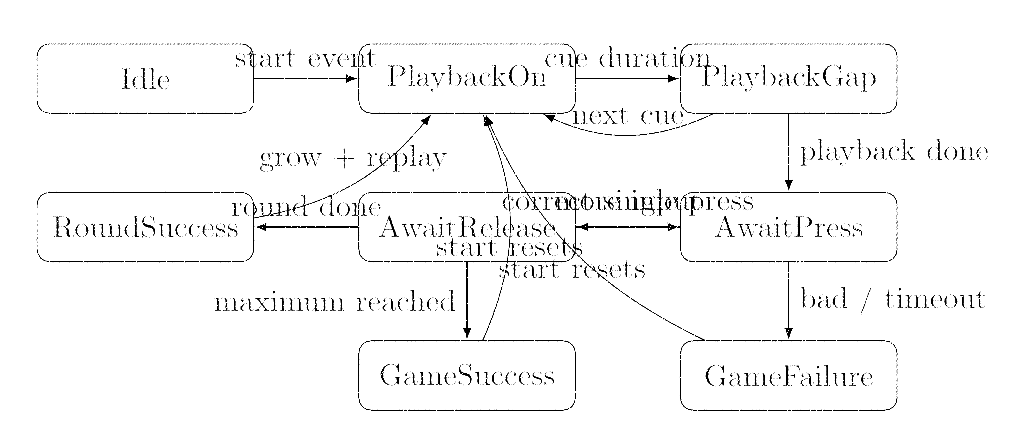
\includegraphics[width=\linewidth,height=0.34\textheight,keepaspectratio]
  {006-simon-state-pencil.png}
\end{center}

\begin{tabularx}{\linewidth}{@{}l X X@{}}
\toprule
Phase & Accepted transition & Snapshot evidence\\
\midrule
Idle & \texttt{startEvent} & sequence length already generated\\
PlaybackOn & cue-on duration due & one \texttt{ledMask} bit; displayed cue valid\\
PlaybackGap & gap due & next cue or \texttt{AwaitPress}\\
AwaitPress & one press, mismatch, chord, or timeout & expected cue and deadline valid\\
AwaitRelease & \texttt{activeMask == 0} & press held until complete release\\
RoundSuccess & result duration due & source grows sequence, then playback\\
GameSuccess / Failure & \texttt{startEvent} & source reset; same sequence repeats\\
\bottomrule
\end{tabularx}

\textbf{Boundary rule.} At a deadline, the deadline transition wins according
to the implementation's branch order. In \texttt{AwaitPress}, timeout is
checked before input. Test a press exactly at the timeout and document the
expected \texttt{Timeout}.

\newpage
\section{Golden replay with a fixed source}

Use the configuration and source from the API listing. The canonical Mega
adapter contains the same bounded fixture behind
\texttt{ADK\_LESSON006\_FIXED\_REPLAY}. Build that exact artifact with:

\begin{lstlisting}[style=adkcpp]
arduino-cli compile --fqbn arduino:avr:mega \
  --build-property compiler.cpp.extra_flags=-DADK_LESSON006_FIXED_REPLAY=1 \
  examples/Lesson006Simon
\end{lstlisting}

The default value is zero and retains the seeded demonstration. Value one
selects only the two-entry \texttt{One}, \texttt{Three} source and the published
100/50/500/100\,ms configuration with maximum length two. Record the define
and resulting binary size with the bench evidence. Each replay-table row is
one engine call; do not invent intermediate ticks when reproducing the host
trace.

\begin{center}
\small
\begin{tabularx}{\linewidth}{@{}r l l X@{}}
\toprule
ms & input change & phase after update & required snapshot fact\\
\midrule
0   & start event & PlaybackOn & displayed One; LED mask \texttt{0x01}\\
99  & none & PlaybackOn & deadline not due\\
100 & none & PlaybackGap & LED mask zero\\
150 & none & AwaitPress & expected One; input accepted\\
200 & One pressed/active & AwaitRelease & observed One; player index 0\\
220 & One released; active zero & RoundSuccess & \texttt{RoundComplete}\\
320 & none & PlaybackOn & length 2; displayed One\\
420 & none & PlaybackGap & LED mask zero\\
470 & none & PlaybackOn & displayed Three; mask \texttt{0x04}\\
570 & none & PlaybackGap & LED mask zero\\
620 & none & AwaitPress & expected One\\
700 & One pressed/active & AwaitRelease & observed One\\
720 & One released; active zero & AwaitPress & expected Three\\
800 & Three pressed/active & AwaitRelease & observed Three\\
820 & Three released; active zero & GameSuccess & \texttt{GameComplete}\\
\bottomrule
\end{tabularx}
\end{center}

\evidencebox{\textbf{Replay proof.} Construct two new sources and games. Feed
both the same rows. After every update compare status, phase, outcome, all cue
presence flags and values, deadline presence/value, LED mask, sequence length,
indices, and input-accepted flag. Final outcome alone is not enough.}

\subsection{Versioned PRNG}

\texttt{XorShift32CueSource} reports
\texttt{SimonAlgorithm::XorShift32V1}. With seed \texttt{0x12345678}, the first
eight internal states are:

\begin{center}
\begin{tabular}{@{}rllllllll@{}}
\toprule
draw & 1 & 2 & 3 & 4 & 5 & 6 & 7 & 8\\
\midrule
state (hex) & 87985aa5 & 155b24a3 & 4820f4c4 & 81b3ac98 &
703a0788 & 29a8e24d & 89ca4f1d & c5186e29\\
cue index & 1 & 3 & 0 & 0 & 0 & 1 & 1 & 1\\
\bottomrule
\end{tabular}
\end{center}

The cue is the low two state bits, mapped 0--3 to One--Four. Verify the vector
exactly. Seed zero is normalized to the documented nonzero seed
\texttt{0x6d2b79f5}; record the value returned by \texttt{seed()}, not merely
the requested value. This generator supports replay, not security or gambling.

\section{Correctness and fault matrix}

\begin{tabularx}{\linewidth}{@{}p{0.29\linewidth}X p{0.14\linewidth}@{}}
\toprule
Case & Required assertion & Result\\
\midrule
fixed golden replay & every snapshot field matches every row & \checkbox{}\\
same PRNG seed twice & identical cues and snapshots & \checkbox{}\\
different seeds & recorded, deterministic vectors; difference not assumed at every draw & \checkbox{}\\
zero seed & normalized seed and vector are stable & \checkbox{}\\
press mismatch & \texttt{GameFailure}/\texttt{Mismatch}; observed cue retained & \checkbox{}\\
exact two-bit host frame & \texttt{InvalidInput}; no order dependence & \checkbox{}\\
input bit 4 & update returns \texttt{InvalidArgument} & \checkbox{}\\
press at timeout & \texttt{Timeout} wins & \checkbox{}\\
held correct button & remains \texttt{AwaitRelease} & \checkbox{}\\
release then next press & advances exactly once & \checkbox{}\\
fixed source exhausted & \texttt{SourceFailure}; status retained & \checkbox{}\\
invalid cue from source & rejected deterministically & \checkbox{}\\
maximum length 32 & capacity succeeds; 33 configuration rejected & \checkbox{}\\
timestamp rollover & elapsed deadlines remain correct & \checkbox{}\\
backward/ambiguous time & update rejects interval beyond half range & \checkbox{}\\
restart after terminal & source reset reproduces sequence & \checkbox{}\\
hardware claim failure & reverse cleanup; all outputs inactive/high impedance & \checkbox{}\\
shutdown in every phase & tone stopped; PWM zero; pins released & \checkbox{}\\
\bottomrule
\end{tabularx}

\textbf{Exercise.} In \texttt{AwaitPress}, set
\texttt{pressedMask = activeMask = 0x03}. Predict status, phase, outcome, and
whether observed cue is present: \blank{4.5in}.

\textbf{Exercise.} A custom source succeeds once and then returns
\texttt{error() == StatusCode::HardwareFailure}. Identify the phase that discovers this for a
starting length of one: \blank{2.0in}. Identify the final outcome:
\blank{1.4in}.

\section{Output policy}

Apply a snapshot only after a successful engine update:

\begin{itemize}
  \item cue LEDs follow bits 0--3 of \texttt{ledMask};
  \item RGB blue means playback, amber means awaiting input, green means
        success, red means failure, and off means idle;
  \item sound frequency maps by cue: 262, 330, 392, and 523 Hz;
  \item cue sound starts only while \texttt{hasDisplayedCue}; success/failure
        sounds are bounded by explicit durations;
  \item on any adapter error, stop sound, set semantic outputs inactive, then
        shut down endpoints to high impedance in reverse initialization order.
\end{itemize}

The engine does not encode colors or musical notes. \texttt{CueId} is neutral,
so another adapter can use vibration, a display, larger protected drivers, or
accessible multimodal feedback without changing game correctness.

\section{Build Simon in visible stages}

Begin with the four Lesson 002 button paths and verify one release-gated event
per press. Add the Lesson 004 cue and RGB outputs and replay the visible
One--Three sequence without sound. Add the Lesson 005 sounder last, then run
the complete fixed replay and observe that cue light, color, and tone agree.
The full payoff is available only after every earlier component stage works.

\paragraph{Physical acceptance boundary.}
Measured bench acceptance remains a separately controlled campaign; this
learner project does not include identity, operator, reviewer, or sign-off
paperwork.
\section{Diagnose from evidence}

\begin{tabularx}{\linewidth}{@{}p{0.24\linewidth}X X@{}}
\toprule
Observation & Likely cause & First safe check\\
\midrule
one button always active & switch rotated, pin grounded, polarity wrong & power off; continuity test\\
one press becomes several & raw sample used as event, adapter mask not cleared & replay bounce trace\\
wrong cue accepted & bit-to-cue map mismatch & fixed One--Four mapping test\\
two presses depend on order & game updated per button instead of per frame & inspect mask construction\\
sequence changes on replay & hidden seed/time or source not reset & log version, normalized seed, inputs\\
cue stays lit in gap & stale snapshot or wrong phase mapping & compare \texttt{ledMask}\\
tone never stops & sounder update omitted or stale command & inspect bounded duration and shutdown\\
RGB color is inverted & common-anode part or duty inversion & disconnect; verify datasheet\\
board resets & short or excess aggregate current & disconnect immediately\\
\bottomrule
\end{tabularx}

\section{Analysis and extensions}

\begin{enumerate}
  \item Explain why \texttt{releasedMask} is recorded even though the current
        \texttt{AwaitRelease} transition uses \texttt{activeMask == 0}.
  \item Change only timestamps so the golden replay crosses
        \texttt{0xffffffff}. Show each unsigned elapsed calculation.
  \item Add difficulty profiles by constructing a new immutable
        \texttt{SimonConfig}; do not mutate live timing midway through a phase.
  \item Design a color-blind mode using position, blink count, and distinct
        tones. RGB color alone must never carry required state.
  \item Add a serial replay recorder. Define a terse, versioned line containing
        time, masks, start event, phase, outcome, LED mask, indices, algorithm,
        and seed.
  \item Replace the four direct LEDs with a shift register in a later lesson.
        Keep \texttt{SimonSnapshot} unchanged and isolate the new timing in the
        output adapter.
\end{enumerate}

\section{Claim, evidence, reasoning}

\textbf{Claim.} The same recorded inputs produce the same complete Simon
behavior, and the Mega adapter gives each phase unambiguous multimodal feedback.

\textbf{Evidence.} Cite the golden replay, PRNG vector, chord and timeout tests,
current calculation, physical mapping trial, and shutdown measurements.\\[3pt]
\blank{0.98\linewidth}\\[8pt]
\blank{0.98\linewidth}\\[8pt]

\textbf{Reasoning.} Connect immutable configuration, explicit timestamps,
complete masks, source reset, snapshot-driven outputs, and RAII cleanup to the
claim. Separate host evidence from hardware observation.\\[3pt]
\blank{0.98\linewidth}\\[8pt]
\blank{0.98\linewidth}\\[8pt]

\section{Further reading}

\begin{itemize}
  \item ADK reference, examples, tests, and complementary HTML:
        \href{https://spincyc.github.io/adk/}{project documentation}
  \item Arduino Mega 2560 Rev3 documentation and schematic:
        \href{https://docs.arduino.cc/hardware/mega-2560/}{official hardware page}
  \item Microchip ATmega2560 electrical and port limits:
        \href{https://www.microchip.com/en-us/product/ATmega2560}{official device page}
  \item Arduino tone and GPIO language references:
        \href{https://docs.arduino.cc/language-reference/}{official language reference}
  \item C++ Core Guidelines resource management:
        \href{https://isocpp.github.io/CppCoreGuidelines/CppCoreGuidelines\#S-resource}{resource section}
  \item Xorshift generator family, George Marsaglia, 2003:
        \href{https://www.jstatsoft.org/article/view/v008i14}{Journal of Statistical Software}
\end{itemize}

\textbf{Review the evidence.}
Explain how the golden replay, chord rejection, current calculation, and safe
shutdown support distinct claims.

\vfill
\begin{center}
\small ADK lesson 006 --- rich printable experiment companion to the terse HTML reference
\end{center}

\end{document}
